\documentclass{article}
\usepackage[margin=1in]{geometry}
\usepackage{amsmath}
\usepackage{amsfonts}
\usepackage{graphicx}
\usepackage{xcolor}
\usepackage{ulem}
\usepackage{hyperref}
% Calligraphic fonts
\newcommand{\calA}{{\cal A}}
\newcommand{\calB}{{\cal B}}
\newcommand{\calC}{{\cal C}}
\newcommand{\calD}{{\cal D}}
\newcommand{\calE}{{\cal E}}
\newcommand{\calF}{{\cal F}}
\newcommand{\calG}{{\cal G}}
\newcommand{\calH}{{\cal H}}
\newcommand{\calI}{{\cal I}}
\newcommand{\calJ}{{\cal J}}
\newcommand{\calK}{{\cal K}}
\newcommand{\calL}{{\cal L}}
\newcommand{\calM}{{\cal M}}
\newcommand{\calN}{{\cal N}}
\newcommand{\calO}{{\cal O}}
\newcommand{\calP}{{\cal P}}
\newcommand{\calQ}{{\cal Q}}
\newcommand{\calR}{{\cal R}}
\newcommand{\calS}{{\cal S}}
\newcommand{\calT}{{\cal T}}
\newcommand{\calU}{{\cal U}}
\newcommand{\calV}{{\cal V}}
\newcommand{\calW}{{\cal W}}
\newcommand{\calX}{{\cal X}}
\newcommand{\calY}{{\cal Y}}
\newcommand{\calZ}{{\cal Z}}

% Sets:
\newcommand{\setA}{\textsf{A}}
\newcommand{\setB}{\textsf{B}}
\newcommand{\setC}{\textsf{C}}
\newcommand{\setD}{\textsf{D}}
\newcommand{\setE}{\textsf{E}}
\newcommand{\setF}{\textsf{F}}
\newcommand{\setG}{\textsf{G}}
\newcommand{\setH}{\textsf{H}}
\newcommand{\setI}{\textsf{I}}
\newcommand{\setJ}{\textsf{J}}
\newcommand{\setK}{\textsf{K}}
\newcommand{\setL}{\textsf{L}}
\newcommand{\setM}{\textsf{M}}
\newcommand{\setN}{\textsf{N}}
\newcommand{\setO}{\textsf{O}}
\newcommand{\setP}{\textsf{P}}
\newcommand{\setQ}{\textsf{Q}}
\newcommand{\setR}{\textsf{R}}
\newcommand{\setS}{\textsf{S}}
\newcommand{\setT}{\textsf{T}}
\newcommand{\setU}{\textsf{U}}
\newcommand{\setV}{\textsf{V}}
\newcommand{\setW}{\textsf{W}}
\newcommand{\setX}{\textsf{X}}
\newcommand{\setY}{\textsf{Y}}
\newcommand{\setZ}{\textsf{Z}}

% Vectors
\newcommand{\bfa}{\mathbf{a}}
\newcommand{\bfb}{\mathbf{b}}
\newcommand{\bfc}{\mathbf{c}}
\newcommand{\bfd}{\mathbf{d}}
\newcommand{\bfe}{\mathbf{e}}
\newcommand{\bff}{\mathbf{f}}
\newcommand{\bfg}{\mathbf{g}}
\newcommand{\bfh}{\mathbf{h}}
\newcommand{\bfi}{\mathbf{i}}
\newcommand{\bfj}{\mathbf{j}}
\newcommand{\bfk}{\mathbf{k}}
\newcommand{\bfl}{\mathbf{l}}
\newcommand{\bfm}{\mathbf{m}}
\newcommand{\bfn}{\mathbf{n}}
\newcommand{\bfo}{\mathbf{o}}
\newcommand{\bfp}{\mathbf{p}}
\newcommand{\bfq}{\mathbf{q}}
\newcommand{\bfr}{\mathbf{r}}
\newcommand{\bfs}{\mathbf{s}}
\newcommand{\bft}{\mathbf{t}}
\newcommand{\bfu}{\mathbf{u}}
\newcommand{\bfv}{\mathbf{v}}
\newcommand{\bfw}{\mathbf{w}}
\newcommand{\bfx}{\mathbf{x}}
\newcommand{\bfy}{\mathbf{y}}
\newcommand{\bfz}{\mathbf{z}}


\newcommand{\bfalpha}{\boldsymbol{\alpha}}
\newcommand{\bfbeta}{\boldsymbol{\beta}}
\newcommand{\bfgamma}{\boldsymbol{\gamma}}
\newcommand{\bfdelta}{\boldsymbol{\delta}}
\newcommand{\bfepsilon}{\boldsymbol{\epsilon}}
\newcommand{\bfzeta}{\boldsymbol{\zeta}}
\newcommand{\bfeta}{\boldsymbol{\eta}}
\newcommand{\bftheta}{\boldsymbol{\theta}}
\newcommand{\bfiota}{\boldsymbol{\iota}}
\newcommand{\bfkappa}{\boldsymbol{\kappa}}
\newcommand{\bflambda}{\boldsymbol{\lambda}}
\newcommand{\bfmu}{\boldsymbol{\mu}}
\newcommand{\bfnu}{\boldsymbol{\nu}}
\newcommand{\bfomicron}{\boldsymbol{\omicron}}
\newcommand{\bfpi}{\boldsymbol{\pi}}
\newcommand{\bfrho}{\boldsymbol{\rho}}
\newcommand{\bfsigma}{\boldsymbol{\sigma}}
\newcommand{\bftau}{\boldsymbol{\tau}}
\newcommand{\bfupsilon}{\boldsymbol{\upsilon}}
\newcommand{\bfphi}{\boldsymbol{\phi}}
\newcommand{\bfchi}{\boldsymbol{\chi}}
\newcommand{\bfpsi}{\boldsymbol{\psi}}
\newcommand{\bfomega}{\boldsymbol{\omega}}
\newcommand{\bfxi}{\boldsymbol{\xi}}
\newcommand{\bfell}{\boldsymbol{\ell}}

% Matrices
\newcommand{\bfA}{\mathbf{A}}
\newcommand{\bfB}{\mathbf{B}}
\newcommand{\bfC}{\mathbf{C}}
\newcommand{\bfD}{\mathbf{D}}
\newcommand{\bfE}{\mathbf{E}}
\newcommand{\bfF}{\mathbf{F}}
\newcommand{\bfG}{\mathbf{G}}
\newcommand{\bfH}{\mathbf{H}}
\newcommand{\bfI}{\mathbf{I}}
\newcommand{\bfJ}{\mathbf{J}}
\newcommand{\bfK}{\mathbf{K}}
\newcommand{\bfL}{\mathbf{L}}
\newcommand{\bfM}{\mathbf{M}}
\newcommand{\bfN}{\mathbf{N}}
\newcommand{\bfO}{\mathbf{O}}
\newcommand{\bfP}{\mathbf{P}}
\newcommand{\bfQ}{\mathbf{Q}}
\newcommand{\bfR}{\mathbf{R}}
\newcommand{\bfS}{\mathbf{S}}
\newcommand{\bfT}{\mathbf{T}}
\newcommand{\bfU}{\mathbf{U}}
\newcommand{\bfV}{\mathbf{V}}
\newcommand{\bfW}{\mathbf{W}}
\newcommand{\bfX}{\mathbf{X}}
\newcommand{\bfY}{\mathbf{Y}}
\newcommand{\bfZ}{\mathbf{Z}}


\newcommand{\bfGamma}{\boldsymbol{\Gamma}}
\newcommand{\bfDelta}{\boldsymbol{\Delta}}
\newcommand{\bfTheta}{\boldsymbol{\Theta}}
\newcommand{\bfLambda}{\boldsymbol{\Lambda}}
\newcommand{\bfPi}{\boldsymbol{\Pi}}
\newcommand{\bfSigma}{\boldsymbol{\Sigma}}
\newcommand{\bfUpsilon}{\boldsymbol{\Upsilon}}
\newcommand{\bfPhi}{\boldsymbol{\Phi}}
\newcommand{\bfPsi}{\boldsymbol{\Psi}}
\newcommand{\bfOmega}{\boldsymbol{\Omega}}


% Blackboard Bold:
\newcommand{\bbA}{\mathbb{A}}
\newcommand{\bbB}{\mathbb{B}}
\newcommand{\bbC}{\mathbb{C}}
\newcommand{\bbD}{\mathbb{D}}
\newcommand{\bbE}{\mathbb{E}}
\newcommand{\bbF}{\mathbb{F}}
\newcommand{\bbG}{\mathbb{G}}
\newcommand{\bbH}{\mathbb{H}}
\newcommand{\bbI}{\mathbb{I}}
\newcommand{\bbJ}{\mathbb{J}}
\newcommand{\bbK}{\mathbb{K}}
\newcommand{\bbL}{\mathbb{L}}
\newcommand{\bbM}{\mathbb{M}}
\newcommand{\bbN}{\mathbb{N}}
\newcommand{\bbO}{\mathbb{O}}
\newcommand{\bbP}{\mathbb{P}}
\newcommand{\bbQ}{\mathbb{Q}}
\newcommand{\bbR}{\mathbb{R}}
\newcommand{\bbS}{\mathbb{S}}
\newcommand{\bbT}{\mathbb{T}}
\newcommand{\bbU}{\mathbb{U}}
\newcommand{\bbV}{\mathbb{V}}
\newcommand{\bbW}{\mathbb{W}}
\newcommand{\bbX}{\mathbb{X}}
\newcommand{\bbY}{\mathbb{Y}}
\newcommand{\bbZ}{\mathbb{Z}}





\title{ECE 417 Midterm 2 2022}
\date{April 1, 2022}
\author{Instructor: Vikas Dhiman \texttt{vikas.dhiman@maine.edu}}

\newtheorem{prob}{Problem}
\newif\ifsol
\solfalse

\begin{document}
\maketitle
%$ \hat{\mathbf{w}} = \hat{\mathbf{k}} \times \frac{\mathbf{v}}{\|\mathbf{v}\|} $
%$ \|\hat{\mathbf{w}}\| = \|\hat{\mathbf{k}}\| \|\frac{\mathbf{v}}{\|\mathbf{v}\|}\| \sin(\phi) $. 

\begin{tabular}{p{0.5\linewidth}p{0.5\linewidth}}
  (1) Student name:& Student email: \\
\end{tabular}

\subsubsection*{About the exam}
\begin{enumerate}
  \item There are total 5 problems. You must attempt all 5. 
  \item Maximum marks: 50 (55 with bonus marks).
  \item Maximum time allotted:  50 min
  \item Calculators are allowed.
  \item One US Letter size or A4 size cheat sheet (both-sides) is allowed.
  \item For all problems, you can assume that the singular value decomposition
    of any matrix is given and you can leave the answer in terms of SVD or
    formula without substituting in the values.
\end{enumerate}

\newcommand{\ubfu}{\underline{\bfu}}
\newcommand{\ubfX}{\underline{\bfX}}
\newpage
\begin{prob}
  Do either problem 1(a) or 1(b). (25 marks)
  \\
  \textbf{Problem 1(a)}:\\
  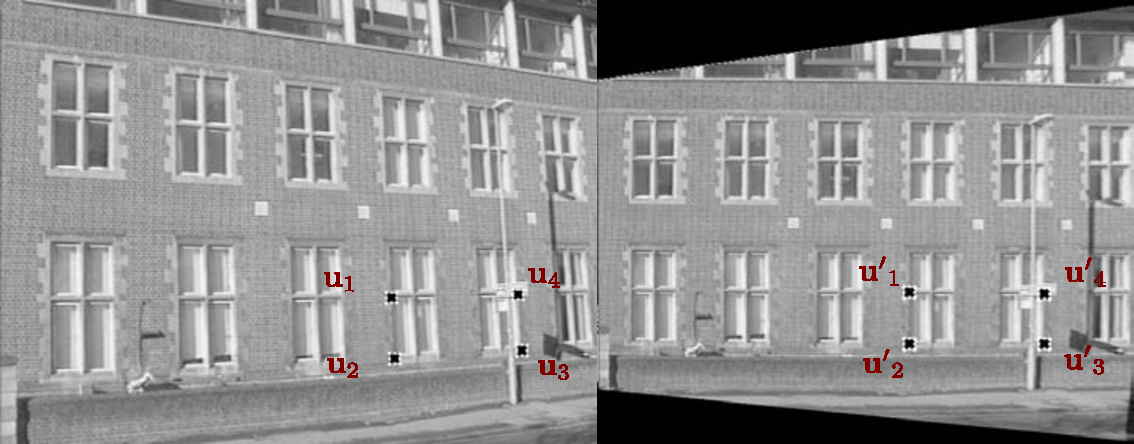
\includegraphics[width=\linewidth]{media/removing-perspective-distortion.png.pdf}
  \begin{align*}
    \ubfu_1 &= [100, 98, 1]^\top&
                                  \ubfu_2 &= [102, 95, 1]^\top\\
    \ubfu_3 &= [107, 90, 1]^\top&
                                  \ubfu_4 &= [110, 85, 1]^\top \\
    \ubfu'_1 &= [100, 98, 1]^\top&
                                   \ubfu'_2 &= [102, 95, 1]^\top\\
    \ubfu'_3 &= [107, 98, 1]^\top&
                                   \ubfu'_4 &= [110, 95, 1]^\top
  \end{align*}
  Find $H$ such that $\ubfu'_i = \lambda_i H\ubfu_i$ for any point on one image to another
  image, where $\ubfu'_i, \ubfu_i \in \bbP^2$ and $\lambda_i \in \bbR$ is a scalar. In other words, convert $\ubfu'_i
  \times H \ubfu_i = 0_{3 \times 1}$ into a system of linear equations that can
  be solved using familiar $A\bfy = 0$ form. For notation purposes, you can use
  $\ubfu_i \in \begin{bmatrix}x_i\\ y_i \\ w_i\end{bmatrix}$,
  $\ubfu'_i \in \begin{bmatrix}x'_i\\ y'_i \\ w'_i\end{bmatrix}$ and $H
  = \begin{bmatrix}
    \bfh_1^\top \\
    \bfh_2^\top \\
    \bfh_3^\top
    \end{bmatrix}$ where $\bfh_1, \bfh_2, \bfh_3 \in \bbR^3$. Cross product
    matrix of vector $\ubfu'_i$ is given as $\ubfu'_i \times = \begin{bmatrix}
      0 & -w'_i & y_i \\
      w'_i & 0 & -x'_i \\
      -y'_i &  x'_i & 0
      \end{bmatrix}$.
  \newpage
  \textbf{Problem 1(b)}:
  Find the 3D position of the
  pothole in the $t+1$ coordinate frame, in terms of $d = 1$ (the movement of the camera),
  image-coordinates of the pothole $\underline{\bfu}_t$, $\underline{\bfu}_{t+1}$ (provided in figure), camera matrix $K$ (provided in figure).
  The car has moved from directly forward along $Z_t$-axis by $d=1$m without any rotation.
  We get two images at time $t$ and at $t+1$. The detection of the pothole at
  time $t$ is $\underline{\bfu}_t = [100, 75, 1]^\top$ and
  $\underline{\bfu}_{t+1} = [100, 95, 1]^\top$.
  Provide the formula or pseudo-code for computing the
  pothole coordinates.  You may or may not need the following equations:
  \begin{enumerate}
    \item Projection of a 3D point $\bfX_c \in \bbR^3$ to an image point $\ubfu
      \in \bbP^2$ by pin hole camera model $\ubfu = K\bfX_c$, where $K$ is the
      camera calibration matrix.
    \item Transforming a coordinate from one coordinate frame to another $X_c =
      ^cR_w X_c  + ^ct_w$ using given rotation matrix $^cR_w$ and translation $^ct_w$ 
    \item The parameteric representation of a 3D line is $\bfx = \lambda \bfd + \bfx_0$,
      where $\bfd \in \bbR^3$ is the direction of the line, $\bfx_0 \in \bbR^3$
      is any point on the line and $\lambda \in \bbR$ is a scalar.
    \end{enumerate}
  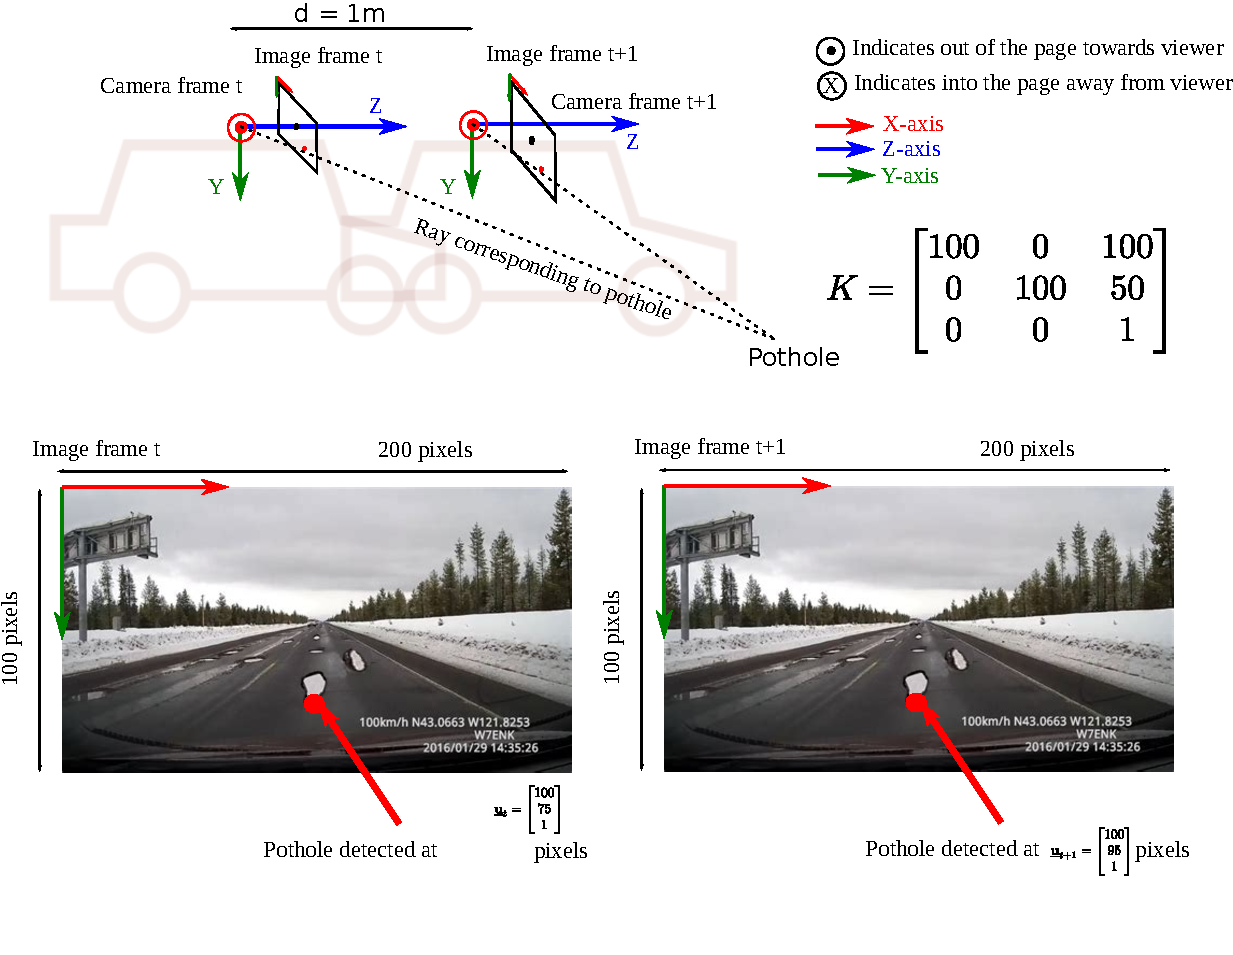
\includegraphics[width=0.7\linewidth]{media/image-road-triangulation-ray-ray.pdf}
\end{prob}

\newpage
.

\newpage
\begin{prob}
  Find the minimum point of the function, $f(\bfy) = \bfy^\top A^\top A (\bfy-\bfd) - \bfy^\top\bfb +
  \bfc^\top \bfy + e$. Let $\bfy \in \bbR^{n \times 1}$ be a n-dimensional
  vector and sizes of $A, \bfb, \bfc, \bfd, e$
  be such that matrix multiplication and addition is valid. Also assume that $A^\top A$  is
  full rank, hence invertible. You may or may not need the following equations,
  \begin{enumerate}
      \item $\frac{\partial }{\partial \bfy} \bfy^\top Q \bfy = 2Q\bfy$.
      \item $\frac{\partial }{\partial \bfy}  \bfq^\top \bfy = \frac{\partial
        }{\partial \bfy}  \bfy^\top \bfq = \bfq$.
  \end{enumerate} (10 marks).
\end{prob}


\newpage
\begin{prob}
  Find the 3D line in parameteric representation that is formed by the intersection of two planes $\bfp^\top \underline{\bfx} = 0$ (with $\bfp = [1, 2,
  3, 4]^\top$)  and $\bfq^\top \underline{\bfx} = 0$ where $\bfq = [-3, 2, 1,
  4]^\top$.
  You may or may not need the following equations,
  \begin{enumerate}
    \item Pseudo-inverse of a tall matrix $A^\dagger = (A^\top A)^{-1} A^\top$.
    \item Pseudo-inverse of a fat matrix $A^\dagger = A^\top(A A^\top)^{-1} $.
  \end{enumerate}
  (10 marks)
\end{prob}

\newpage
\begin{prob}
  Find the point on the intersection of following 3D lines $\bfx = \lambda_1
  \bfd_1 +  \bfx_1$ and $\bfx = \lambda_2 \bfd_2 + \bfx_2$. Here $\lambda_1\in \bbR$ and
  $\lambda_2 \in \bbR$ are the free parameters. The rest of the parameters have
  the following values
  \begin{align*}
    \bfd_1 = [1, 2, 0]^\top,
    \bfd_2 = [-2, 1, 0]^\top,
    \bfx_1 = [1, 2, 0]^\top,
    \bfx_2 = [4, 5, 0]^\top.
    \end{align*} 
    You may or may not need the following equations,
    \begin{enumerate}
    \item Pseudo-inverse of a tall matrix $A^\dagger = (A^\top A)^{-1} A^\top$.
    \item Pseudo-inverse of a fat matrix $A^\dagger = A^\top(A A^\top)^{-1} $.
    \end{enumerate} (10 marks).
\end{prob}

\newpage
\begin{prob}
  Find the point of intersection of the 3D line $\bfx = \lambda \bfd + \bfx_0$ with
  the 3D plane $\bfp^\top \underline{\bfx} = 0$. The parameters have the
  following values
  \begin{align*}
    \bfd = [1, 2, 0]^\top, \bfx_0 = [3, 4, 5]^\top, \bfp = [1, 2, 0, 7]^\top.
  \end{align*} (10 marks).
\end{prob}


\end{document}
